\section{} \label{sec:1}
\quest{Határozzuk meg, hogy egy szobahőmérsékleten levő, ideálisnak tekinthető gázban mennyi
idő alatt jut el egy CO molekula a szoba egyik végéből a másikba tisztán diffúz mozgással.
\\ \\
Segítség: \\
A kinetikus elmélet a gázok diffúziós együtthatójára a következő kifejezést adja (és az
eredményt érthetjük is a Brown-mozgásról tanultak alapján):
\begin{equation*}
    D
    =
    \frac{1}{3} l \left< v \right>
    \quad \quad
    \left(
    = \frac{\left( \Delta x \right)^{2}}{2 \tau}
    \approx
    \frac{l^{2}}{\tfrac{3 l}{\left< v \right>}}
    \right)
\end{equation*}
ahol $l$ a molekulák szabad úthossza, $\left< v \right>$ pedig átlagos sebességük. A szabad úthosszt megbecsülhetjük a $l = \tfrac{1}{n \pi d^{2}}$ kifejezésből, ahol $n$ a molekulák koncentrációja és $d$ a molekulák átmérője. Az átlagos sebességet pedig az ekvipartíció tételéből számolhatjuk. \\
A valóságban a szagok sokkal gyorsabban terjednek egy szobában. Értjük ezt?}

\subsection{Szagok terjedése} \label{sub:1.1}
Először tisztázzuk az utolsó kérdést, ugyanis több, a továbbiakban is felhasználható dologra világít rá annak megválaszolása. \\
A kurzus során a diffúzió leírásának eddig vizsgált elméletei arra a feltételezésre alapulnak, hogy a kérdéses diffundáló anyagot körülvevő közeg részecskéi teljesen véletlenszerű módon mozognak. Az ilyen rendszerek esetére tárgyaltuk az eddigiekben a Brown-mozgás, Einstein- és a Langevin-féle leírását is. Azonban egy valóságos fizikai rendszerben - mint pl. egy átlagos szoba - sokkal több egyéb folyamat is hatással van a levegőben levő részecskék mozgására. \\
A jelen feladat további részében egyedül a hőmérséklet - tehát a közeg részecskéinek hőmozgása - okozta komponens hozzájárulását kell kiszámítanunk, azonban a valóságban mindenhol előforduló, és nagyságrendekkel erősebb konvektív áramlásokat nem vesszük figyelembe. Egy szobában a szagok gyors terjedésének oka csak kis részben függ magától az eddig tárgyalt diffúziós hatásoktól, döntő mértékben az adott közegben - itt levegőben - található áramlatok határozzák azt meg. Ezek kialakulásának oka az egyes térfogatrészekben létrejövő nyomáskülönbségek, melyek a nyitott térben intenzív mennyiség módjára, erőteljes anyagmozgás során egyenlítődnek ki. A nagyobb részecskéket - amiket szagokként érzékelünk - pedig ezek az áramlatok juttatják el gyorsan, nagy távolságra.

\subsection{Előzetes megjegyzések} \label{sub:1.2}
A segítségben megadott összefüggések alapján könnyűszerrel megkaphatjuk a diffúziós együttható értékének kiszámításához szükséges $l$ és $\left< v \right>$ mennyiségeket. Azonban ennek ellenére vezessük le őket a teljes képért cserébe. \\
Ezekhez előbb szükségünk van az $n$, $d$ értékek megbecslésére, valamint az ekvipartíció tételének alkalmazására. Kezdjük a szabad úthossz kiszámításával!

\subsection{Szabad úthossz} \label{sub:1.3}
A kinetikus gázelméletben egy részecske közepes szabad úthosszának azt a távolságot nevezzük, amennyit átlagosan két, más részecskével történő ütközés között megtesz. Ezt alábbi formula fejezi ki:

\begin{equation} \label{eq:1}
    l
    =
    \left( \sigma n \right)^{-1}
\end{equation}
Ahol $n$ a közeg részecskéinek koncentrációja, $\sigma$ pedig az ütközéshez tartozó effektív hatáskeresztmetszet. Feltételezve, hogy a közeg ideális gáz, a koncentráció egyszerűen kifejezhető az alábbi módon az általános gáztörvény segítségével:

\begin{equation} \label{eq:2}
    n
    =
    \frac{N}{V} = \frac{p}{k_{B} T}
\end{equation}
Az effektív hatáskeresztmetszet gömb alakú, $r$ sugarú részecskékre az alábbi\cite{meanfreepath} módon írható fel:

\begin{equation} \label{eq:3}
    \sigma
    =
    \pi * \left( 2 r \right)^{2}
    =
    \pi d^{2}
\end{equation}
Amely alakból a segítségben is ismertetett nevező lesz a végleges egyenletünkben. A kettő behelyettesítve az eredeti (\ref{eq:1})-es egyenletbe, a következőt kapjuk:

\begin{equation} \label{eq:4}
    l
    =
    \left( \frac{p}{k_{B} T} * \pi d^{2} \right)^{-1}
    =
    \boxed{\frac{k_{B} T}{p \pi d^{2}}}
\end{equation}
Melyben $T$ és $p$, légköri nyomást és szobahőmérsékletet feltételezve ismert, $d$ pedig becsülhető a CO molekula paramétereinek ismeretében. Ennek konstitúciós képlete az alábbi egyszerű struktúra:

\begin{figure}[h]
    \centering
    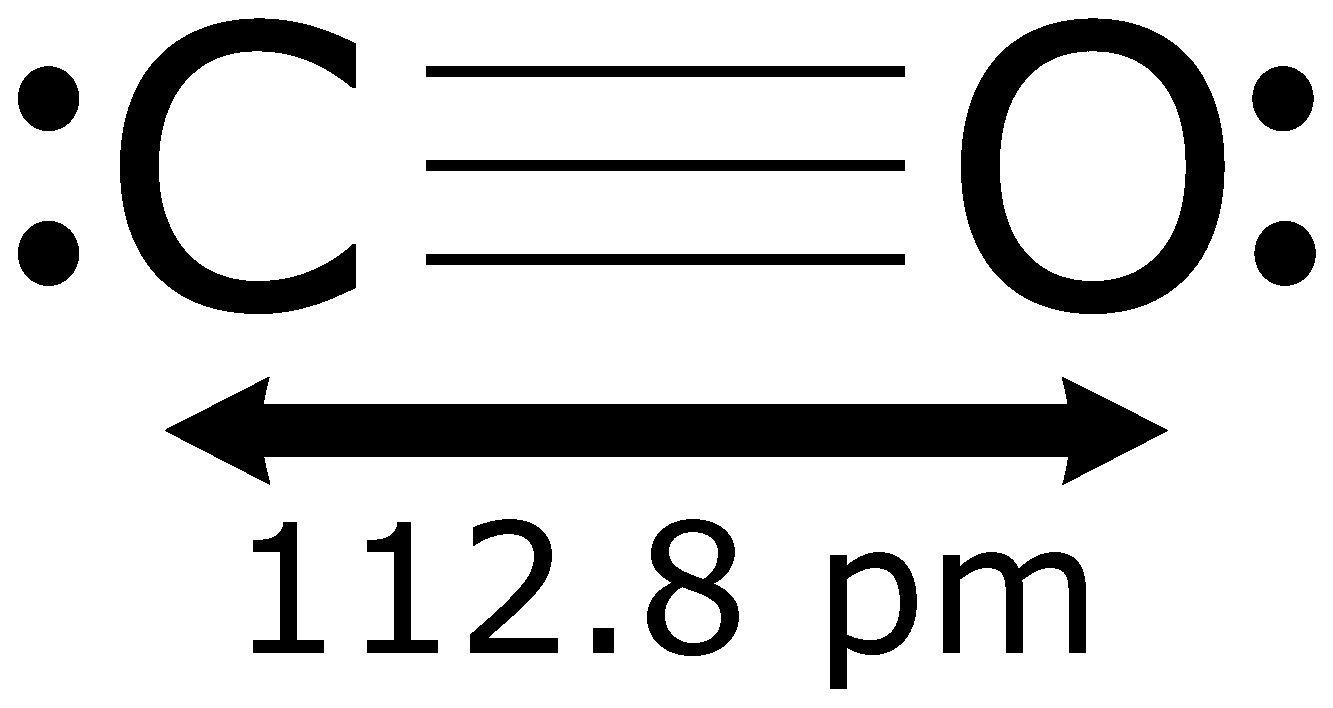
\includegraphics[width=.2\textwidth]{images/Carbon_monoxide_2D.eps}
    \caption{Structure diagram of carbon monoxide (CO)}
    \label{fig:1}
\end{figure}

Melynek a képen is bejelölt hosszirányú nagysága $112.8\ \text{pm} = 1.128 * 10^{-10}\ \text{m}$. Ha ezt a molekulát gömbként közelítjük, ezt az értéket vehetjük ezen gömb $d$ átmérőjének. \\
A légköri nyomás általánosan is használt értéke $101\,325\ \text{Pa}$, míg a szobahőmérséklet $25.0\ ^{\circ}\text{C} = 298\ \text{K}$. Ezek felhasználásával már kiszámítható a CO molekula szabad úthossza, a (\ref{eq:4})-es egyenletbe történő behelyettesítéssel:

\begin{equation}
    l
    =
    \frac{ 1.3806 * 10^{-23}\ \frac{\text{kg m}^{2}}{\text{K s}^{2}} * 298\ \text{K}} { 101\,325\ \text{Pa} * \pi * \left( 1.128 * 10^{-10}\ \text{m} \right)^{2}}
    =
    \boxed{1.01578 * 10^{-6}\ \text{m}}
\end{equation}
A szabad úthossz dimenzióját egy egyszerű számítással ellenőrizzük:

\begin{equation}
    \left[ l \right]
    =
    \frac{\dfrac{\text{kg m}^{2}}{\text{K s}^{2}}\text{K}}{\text{Pa} * \text{m}^{2}}
    =
    \frac{\dfrac{\text{kg m}^{2}}{\text{K}\ \text{s}^{2}}\text{K}}
         {\dfrac{\text{kg}}{\text{m}\ \text{s}} * \text{m}^{2}}
    =
    \frac{\dfrac{\cancel{\text{kg m}^{2}}}{\cancel{\text{K}}\ \cancel{\text{s}^{2}}} \cancel{\text{K}}}
         {\dfrac{\cancel{\text{kg}}}{\text{m}\ \cancel{\text{s}^{2}}} * \cancel{\text{m}^{2}}}
    =
    \frac{1}{\frac{1}{\text{m}}}
    =
    \text{m}
\end{equation}
Vagyis fentebb a helyes eredményt kaptuk meg a szabad úthosszra. Ellenőrizve a szakirodalomban azt találjuk\cite{mfponsealevel}\cite{jennings1988mean}, hogy nagyjából a tengerszinten, levegőben egy részecske átlagos szabad úthossza $0.001\ \text{$\mu$m} - 0.1\ \text{$\mu$m}$, ami nagyságrendileg megegyezik az itt kapott eredménnyel.

\subsection{A részecskék sebessége} \label{sub:1.4}
Az átlagos sebesség az ekvipartíció-tétel alapján számítható, mely a következőt mondja ki a részecskék kinetikus energiájának várható értékére:

\begin{equation} \label{eq:7}
    \left< \mathrm{H}_{\text{kin}} \right>
    =
    \frac{\left< p_{x}^{2} + p_{y}^{2} + p_{z}^{2} \right>}{2m}
    =
    \frac{m^{\cancel{2}} \left< v_{x}^{2} + v_{y}^{2} + v_{z}^{2} \right>}{2\cancel{m}}
    =
    \frac{1}{2} m * \left< v_{x}^{2} + v_{y}^{2} + v_{z}^{2} \right>
    =
    \frac{3}{2} k_{B} T
\end{equation}
Tehát végérvényesen a részecskék átlagsebességének négyzetéről azt mondhatjuk, hogy

\begin{equation} \label{eq:8}
    \left< v_{x}^{2} + v_{y}^{2} + v_{z}^{2} \right>
    =
    \left< \boldsymbol{v} * \boldsymbol{v} \right>
    =
    \left< v^{2} \right>
    =
    \frac{3 k_{B} T}{m}
    \quad \to \quad
    \boxed{v = \sqrt{\frac{3 k_{B} T}{m}}}
\end{equation}
Behelyettesítve a CO molekula tömegét 
\begin{equation}
    m_{CO}
    =
    \frac{28.01\ \frac{\text{g}}{\text{mol}}}{N_{A}}
    =
    \frac{28.01\ \frac{\text{g}}{\text{mol}}}{6.02214 * 10^{23}\ \frac{1}{\text{mol}}}
\end{equation}
Valamint a $T = 298\ \text{K}$ szobahőmérsékletet a (\ref{eq:8}).as egyenletbe a következőt kapjuk:

\begin{align}
    \left< v \right>
    &=
    \sqrt{\frac{3 k_{B} T}{m}}
    =
    \sqrt{\frac{3 k_{B} * 298\ \text{K}}{\frac{28.01\ \frac{\text{g}}{\cancel{\text{mol}}}}{6.02214 * 10^{23}\ \cancel{\frac{1}{\text{mol}}}}}}
    =
    \sqrt{\frac{3 k_{B} * 298\ \text{K} * 6.02214 * 10^{23}}{28.01\ \text{g}}} = \nonumber \\
    &=
    \sqrt{\frac{3 * 1.3806 * \cancel{10^{-23}}\ \frac{\text{kg m}^{2}}{\text{K s}^{2}} * 298\ \text{K} * 6.02214 * \cancel{10^{23}}}{28.01\ \text{g}}} = \nonumber \\
    &=
    \sqrt{\frac{3 * 1.3806\ \frac{\text{\cancel{kg} m}^{2}}{\text{\cancel{K} s}^{2}} * 298\ \cancel{\text{K}} * 6.02214}{2.801 * 10^{-2}\ \cancel{\text{kg}}}}
    =
    \sqrt{\frac{3 * 1.3806 * 298 * 6.02214}{2.801 * 10^{-2}}}\ \frac{\text{m}}{\text{s}} \approx \nonumber \\
    &\approx
    \sqrt{265\,364.685}\ \frac{\text{m}}{\text{s}}
    \approx
    \boxed{515.14\ \frac{\text{m}}{\text{s}}}
\end{align}

Ennyi a CO molekulák átlagos sebessége a levegőben, standardállapotban.

\subsection{A diffúziós együttható}
A két végeredmény behelyettesítésével végre kifejezhetjük a diffúziós együtthatót:

\begin{align}
    D
    &=
    \frac{1}{3} l \left< v \right>
    =
    \frac{1}{3} * 1.01578 * 10^{-6}\ \text{m} * 515.14\ \frac{\text{m}}{\text{s}} = \nonumber \\
    &=
    \frac{1}{3} * 1.01578 * 10^{-6} * 515.14\ \frac{\text{m}^{2}}{\text{s}}
    \approx
    0.0001744\ \frac{\text{m}^{2}}{\text{s}}
    =
    \boxed{1.744\ \frac{\text{cm}^{2}}{\text{s}}}
\end{align}
Ez érdekes módon éppen megegyezik a hidrogén, $200\ ^{\circ}\text{C}$-on mért diffúziós együtthatójával, azonban majdnem $10$-es szorzóval eltér a standarállapoton és szobahőmérsékleten mérhető - és általunk egyébként is keresett - szén monoxidétól, ami $0.208\ \frac{\text{cm}^{2}}{\text{s}}$\cite{diffusivity}. Ennek oka feltehetően az az erős közelítés, miszerint az elnyúlt, hosszúkás CO molekulát egy $d$ átmérőjű gömbként kezeltem, vagy hogy egész egyszerűen egy $10$-es szorzót elvesztettem a számításokban.
\\ \\
A további számításokban tegyük fel, hogy a szoba $5\ \text{m}$ hosszú, a részecskének pedig ezt a távot kell megtennie. A diffúziós együttható kifejezhető a $\left( \Delta x \right)^{2}$ elmozdulásnégyzet értékével, ahol most $\left( \Delta x \right)^{2} = 25\ \text{m}^{2}$. Az alábbi azonosságot írhatjuk fel tehát a segítség alapján:

\begin{equation}
    D
    =
    \frac{\left( \Delta x \right)^{2}}{2 \tau}
    \quad \to \quad
    \tau
    =
    \frac{\left( \Delta x \right)^{2}}{2D}
\end{equation}
Ha a fenti, $D$-re kapott eredménnyel számolunk tovább, akkor a $\tau$ értékére a következőt kapjuk:

\begin{equation}
    \tau
    =
    \frac{\left( \Delta x \right)^{2}}{2D}
    =
    \frac{25\ \cancel{\text{m}^{2}}}{2 * 0.0001744\ \frac{\cancel{\text{m}^{2}}}{\text{s}}}
    =
    \frac{25}{2 * 0.0001744}\ \text{s}
    \approx
    \boxed{
    71674\ \text{s}
    \approx
    0.83\ \text{nap}
    }
\end{equation}
Vagyis kizárólagosan a diffúzió hatására ennyi időbe telne, míg egy CO molekula eljutna a szoba egyik végéből a másikba. A (\ref{sub:1.1})-es pontban pedig szó volt róla, hogy ez miért nem így történik a valóságban.